%%----------------------------------------------------------------------
%%----------------------------------------------------------------------
\missiontitle{Mission: Shuttle Crash\single}

\teaser{A courier shuttle has been shot down, you must seize the pilot
  and their databanks!}

\begin{tablesetup}

  \dawnofwar

  \smallskip%
  After all deployment concludes, randomly determine a table corner.
  Place a flying shuttle marker~12''x12'' from that corner, adjusting
  its position by the minimum distance necessary toward table center
  to not overlap models or impassible terrain.  Models may move under
  the shuttle model and over or onto its base.
\end{tablesetup}

%%----------------------------------------------
\begin{missionrules}
\vspace{-1.5em}%
\noindent%
  \begin{minipage}[t]{\linewidth-(1.75in+1em)}\vbox to 0pt{}
    \textbf{Shuttle Crash.} At the start of game turn~2, either player
    rolls a~D6.  On a~1--2 the shuttle marker scatters toward the
    diagonally opposite table corner, on a~3--4 it scatters toward the
    center of one of the farther opposing table edges, and on a~5--6
    it scatters toward the center of the other farther opposing table
    edge, as shown to the right. The shuttle scatters~3D6 in that
    direction and becomes crashed.

    \smallskip\hspace{1em} Next, place~4 debris markers,~12+2D6'' from
    the shuttle's final position toward each of the~four table
    corners, rolling the distance for each separately.

    \smallskip\hspace{1em} Neither shuttle nor debris will crash onto
    impassable terrain.  Adjust their final positions by the minimal
    necessary distance to prevent this.
  \end{minipage}\hfill
  \begin{minipage}[t]{1.75in}\vbox to 0pt{}
  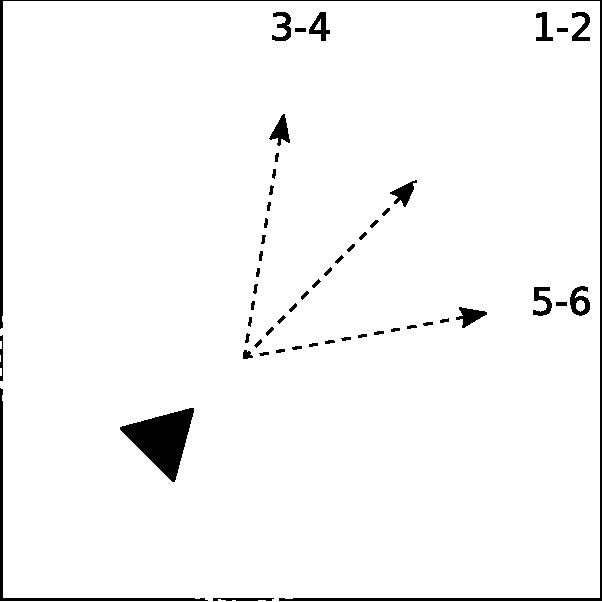
\includegraphics[width=\linewidth]{missions/shuttle-scatter}
  \end{minipage}

  \smallskip Any non-vehicle models under the shuttle or debris
  markers' final positions must pass an initiative test or take a
  wound. Vehicles under such a marker take an~S8 hit on their side
  armor.  Cover saves are not permitted for either but armor and
  invulnerable saves are.  Surviving models are displaced the minimum
  necessary distance to not overlap any marker, model, or impassable
  terrain.

  \smallskip The crashed shuttle and debris act as objective markers,
  dangerous terrain, and give a~5+ cover save.

  \missionsubheading{Wounded Pilot.} At the end of the first movement
  phase in which at least one non-vehicle model is in base contact
  with or on the crashed shuttle marker, the current player places a
  Pilot in base contact with any such model of their choice.  The
  Pilot joins that unit unless forbidden by the latter's rules.

  \begin{center}    
  \begin{tabular}[t]{O{0.75in}ccccccccF{.25in}F{1in}E{2in}}
    & {\bf WS} &  {\bf BS} & {\bf S} & {\bf T} & {\bf W} & {\bf I} & {\bf A} & {\bf Ld} & {\bf Sv} & {\bf Type} & {\bf Special Rules}\\
\hline
    {\bf Pilot} & 3 & - & 3 & 3 & 2 & 2 & - & 7 & 5+ 6++ & Infantry & Neutral NPC\\
  \end{tabular}
  \end{center}

  \hfill
  \begin{minipage}{6in}
    \missionsubheading{Neutral NPC.} See
    page~\pageref{rule:neutral-npc} of this mission book.
  \end{minipage}
  \hfill\hbox to 0pt{}

  % \missionsubheading{Debris.}  Any uncontested debris marker that
  % begins the movement phase in base contact with at least two infantry
  % models from a single unit may be carried up to~6'' by those models
  % as they move, ending the move in base contact with both models.
  % Designate two before moving if there are multiple models in base
  % contact.  No unit can carry more than one debris marker at a time,
  % and any unit that carries a debris marker cannot run or charge that
  % turn.  Debris markers may embark and disembark a transport or
  % building with their carrying models; they are considered bulky.  In
  % no case can a debris marker move more than~6'' in the movement
  % phase, or move at all in any other phase.  In the rare chance that a
  % carrying model is removed as a casualty while moving, i.e., by
  % moving in dangerous terrain, the marker is placed where the final
  % wound occurred.
\end{missionrules}


%%----------------------------------------------
\begin{scoring}  
\begin{primaries}

  At game end if the Wounded Pilot is joined with a unit, then that
  player has captured or rescued them and earns~3 victory points.
  Control of the crashed shuttle is worth~2 victory points at game end
  and each debris marker~1 point.

%\underline{No more than~9 victory points may be earned by primary objectives.}

\end{primaries}
\end{scoring}
